% =====================================================================
%  PHẦN: GIỚI THIỆU GAME TETRIS (lịch sử, ý tưởng game)
%  Người viết: Nguyễn Việt Lâm
% =====================================================================

\providecommand{\khoitetromino}[2]{%
  \foreach \x/\y in {#1}{%
    \draw[fill=black!#2,line width=0.6pt] (\x*0.5,\y*0.5) rectangle ++(0.5,0.5);}}

\subsection{Lịch sử ra đời}

Tetris là một trò chơi xếp hình ra đời tại Moscow, Liên Xô, vào giữa thập niên 1980. Tác giả của game là Alexey Pajitnov, một kỹ sư phần mềm làm việc tại Trung tâm Tính toán thuộc Viện Hàn lâm Khoa học Liên Xô, chuyên nghiên cứu về nhận dạng giọng nói. Ngoài giờ làm việc, ông thường viết những trò chơi nhỏ trên chiếc máy tính Elektronika 60 của viện để thử khả năng của máy, đồng thời để mọi người xung quanh có thêm niềm vui~\cite{tetris_wiki,tetris_myjoy}.

Ý tưởng của Tetris xuất phát từ một món đồ chơi thời thơ ấu của Pajitnov: bộ xếp hình \textit{pentomino}. Trong bộ đồ chơi này, người chơi phải sắp xếp 12 mảnh ghép, mỗi mảnh được tạo từ 5 ô vuông, vào vừa khít một chiếc hộp. Vào tháng 6 năm 1984, ông nảy ra ý định đưa trò xếp hình này lên máy tính. Tuy nhiên, việc cho 12 loại mảnh ghép xoay và rơi theo thời gian thực quá phức tạp, nên ông rút gọn lại còn các mảnh ghép chỉ gồm 4 ô vuông, gọi là \textit{tetromino}~\cite{guardian_tetris,tetris_wiki}. Cái tên \textit{Tetris} được ghép từ ``\textit{tetra}'' (tiếng Hy Lạp nghĩa là bốn) và ``\textit{tennis}'' (môn thể thao yêu thích của tác giả)~\cite{filfre_tetris}.

Phiên bản đầu tiên rất đơn sơ. Chiếc Elektronika 60 chỉ hiển thị được chữ, không có đồ họa, nên các khối gạch phải được vẽ bằng những ký tự như dấu ngoặc vuông. Dù vậy, game nhanh chóng khiến các đồng nghiệp của Pajitnov mê mẩn, ai chơi thử cũng khó rời máy. Sau đó, với sự giúp đỡ của Dmitry Pavlovsky và Vadim Gerasimov, Tetris được chuyển sang máy tính IBM PC phổ biến hơn. Trò chơi lan truyền trong giới lập trình viên chủ yếu qua việc chép lại trên đĩa mềm và truyền miệng, rồi dần ra khỏi biên giới Liên Xô~\cite{denofgeek_tetris,tetris_myjoy}.

Sau nhiều năm tranh chấp bản quyền phức tạp, Tetris được phát hành ở phương Tây và nổi tiếng toàn cầu nhất là nhờ bản Game Boy của Nintendo năm 1989. Đến năm 1996, quyền sở hữu game trở về tay Pajitnov; ông cùng Henk Rogers thành lập The Tetris Company để quản lý việc cấp phép cho các phiên bản chính thức~\cite{tetris_wiki,tetris_myjoy}. Cho đến nay, Tetris đã xuất hiện trên hơn 65 nền tảng khác nhau và có hơn nửa tỷ lượt tải trên thiết bị di động, theo thống kê của The Tetris Company~\cite{tetris_myjoy}.

\subsection{Ý tưởng của game}

Ý tưởng của Tetris đơn giản đến mức chỉ cần xem vài giây là hiểu: các khối gạch rơi dần xuống từ phía trên màn hình, người chơi xoay và di chuyển chúng để xếp thành những hàng ngang kín, không còn khoảng trống. Mỗi hàng kín sẽ biến mất và người chơi được cộng điểm. Nếu các khối chất cao chạm tới đỉnh màn hình thì trò chơi kết thúc.

Mọi khối gạch trong Tetris đều là \textit{tetromino}, tức hình được ghép từ đúng 4 ô vuông nối với nhau theo cạnh. Với cách ghép này chỉ có 7 hình dạng khác nhau, thường được gọi theo hình dáng của chúng là I, O, T, S, Z, J và L (Hình~\ref{fig:bay_tetromino}). Trong bản tiêu chuẩn hiện nay, khu vực chơi là một cột dọc rộng 10 ô và cao 20 ô.

\begin{figure}[H]
\centering
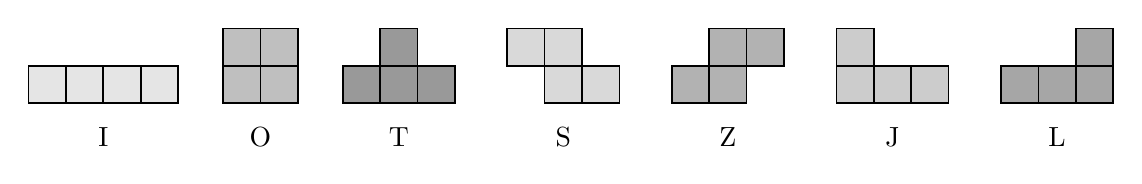
\begin{tikzpicture}[scale=0.95]
  \begin{scope}[shift={(0,0)}]
    \khoitetromino{0/0,1/0,2/0,3/0}{10}
    \node at (1,-0.45) {I};
  \end{scope}
  \begin{scope}[shift={(2.6,0)}]
    \khoitetromino{0/0,1/0,0/1,1/1}{25}
    \node at (0.5,-0.45) {O};
  \end{scope}
  \begin{scope}[shift={(4.2,0)}]
    \khoitetromino{0/0,1/0,2/0,1/1}{40}
    \node at (0.75,-0.45) {T};
  \end{scope}
  \begin{scope}[shift={(6.4,0)}]
    \khoitetromino{1/0,2/0,0/1,1/1}{15}
    \node at (0.75,-0.45) {S};
  \end{scope}
  \begin{scope}[shift={(8.6,0)}]
    \khoitetromino{0/0,1/0,1/1,2/1}{30}
    \node at (0.75,-0.45) {Z};
  \end{scope}
  \begin{scope}[shift={(10.8,0)}]
    \khoitetromino{0/0,1/0,2/0,0/1}{20}
    \node at (0.75,-0.45) {J};
  \end{scope}
  \begin{scope}[shift={(13.0,0)}]
    \khoitetromino{0/0,1/0,2/0,2/1}{35}
    \node at (0.75,-0.45) {L};
  \end{scope}
\end{tikzpicture}
\caption{Bảy khối tetromino trong game Tetris}\label{fig:bay_tetromino}
\end{figure}

Sức hấp dẫn của Tetris nằm ở chỗ luật chơi rất ít nhưng tình huống thì gần như không lặp lại. Các khối xuất hiện ngẫu nhiên, nên mỗi lượt người chơi phải quan sát nhanh, quyết định đặt khối vào đâu và xoay theo hướng nào sao cho không để lại các lỗ trống khó lấp. Khi trò chơi tiến triển, các khối rơi nhanh hơn, tạo ra áp lực tăng dần: chơi giỏi hơn thì càng được thử thách nhiều hơn. Chính sự kết hợp giữa luật chơi dễ học, tốc độ tăng dần và cảm giác thỏa mãn mỗi khi một hàng biến mất khiến Tetris dễ chơi nhưng khó dừng~\cite{filfre_tetris}.

\subsection{Sức ảnh hưởng của Tetris}

Hơn bốn thập kỷ sau khi ra đời, Tetris vẫn được xem là một trong những trò chơi điện tử nổi tiếng và được chơi rộng rãi nhất thế giới. Game có mặt trên máy tính, máy chơi game cầm tay, máy console và điện thoại thông minh, được người chơi ở mọi lứa tuổi yêu thích. Sự thành công này cho thấy một ý tưởng đơn giản, được thiết kế khéo, có thể tồn tại lâu hơn nhiều so với những trò chơi dùng đồ họa và công nghệ phức tạp.

Với nhóm chúng tôi, đây cũng là lý do Tetris là một đề tài phù hợp: luật chơi rõ ràng, dễ hình dung, nhưng khi lập trình lại chứa nhiều bài toán thú vị như điều khiển khối rơi, xoay khối, kiểm tra va chạm và xóa hàng. Phần giới thiệu này là nền tảng để các phần tiếp theo trình bày cách chơi và các chức năng chính mà game của nhóm hướng tới.
